\section{ELSE}
Um die Blickrichtung möglichst exakt zu bestimmen, sind die Landmarks der Pupille ausschlaggebend. Zu diesem Zwick kann ElSe eingesetzt werden, da dies ein Verfahren zur Detektion von Pupillen in Bildern unter realen Bedingungen ist.
\subsection{Funktion}
Das Verfahren ist in der Lage aus Bildern die Umrisse einer Pupille zu ermitteln. Bei realen Aufnahmen sind Bildfehler unvermeidlich, so können Reflektionen (Brille, Kontaktlinse usw.), Make-Up und körperliche Eigenschaften wie Augenfarbe die Detektion erschweren.\\
Als Ergebnis liefert ElSe eine Ellipse, die den Umriss der Pupille beschreibt.
\subsection{Funktionsablauf}
Als Input wird im Orginal ein Graubild einer Eye-Tracking-Brille verwendet, auf dem das Infrarot beleuchtete Auge abgebildet ist. Die Infrarotbeleuchtung wird verwendet, damit das Auge ausreichend beleuchtet ist ohne den Probanden zu blenden. Für den Test im Vergleich zu anderen Verfahren, wurden Bilder von $384\times 288$ Pixel Größe verwendet und ist auf diesen zu einer Echtzeitauswertung fähig.
\subsubsection{Kantendetektion}
Da die Pupille als schwarzen Fleck im Bild dargestellt ist und die Iris einen helleren Farbton aufweist, wird ein Kantendetektor verwendet, der alle Pixel markiert, bei denen eine starke Farbänderung auftritt. Bei ElSe wird ein Morphologischen Ansatz eingesetzt, von Relevanz sind nur zusammenhängende Kantenpixel um die Kante zwischen Pupille und Iris zu finden, alle anderen können ignoriert werden. Wobei jedes Kantenpixel als Startpunkt der Berechnung dienen kann.
\subsubsection{Bestimmen der Ellipse}
Um jene Kantenpixel zu erhalten, die die Pupille beschreiben, wird versucht fortlaufende Kanten zu finden, die eine Ellipse bilden. Jene die nicht diesen Anforderung entsprechen können recht schnell ignoriert werden. Anschließend können auch alle offenen Ellipsenverläufe und jene die am meisten vom bestimmten Verlauf abweichen, verworfen werden.\\
Das beste Ergebnis aller bestimmten Ellipsen wird als Lösung verwendet.
\subsubsection{Grobe Bestimmung der Pupille}
Sollte die Bestimmung der Ellipse, wie im letzten Kapitel beschreiben, scheitern, so wird das Zentrum des dunkelsten Kreises ermittelt. So ein Punkt kann immer gefunden werden, ist aber nicht zwingend die Pupille.\\
Auf einem verkleinertem Bild \autoref{img_else} (1) wird ein kreisförmiger Mean-Filter eingesetzt mit Ergebnis in \autoref{img_else} (3). Zur zweiten Faltung wird der Durchschnitt über ein Quadrat ohne inneren Kreis eingesetzt bestimmt mit Ergebnis in \autoref{img_else} (2), wobei beides mal der selbe Radius verwendet wird.\\
Nun wird das Ergebnis des Quadratischen Mean-Filters invertiert \autoref{img_else} (4) und mittels Punkt-Multiplikation mit dem anderen Meanfilter zusammengebracht \autoref{img_else} (5). Im resultierendem Bild wird nun der höchste Wert gesucht, da dies das Zentrum des dunkelsten kreisförmigen Ortes im Bild ist.\\
Ergebnis des Beispiels ist als Kreuz in \autoref{img_else} (6) markiert. 
\begin{figure}
	\centering
	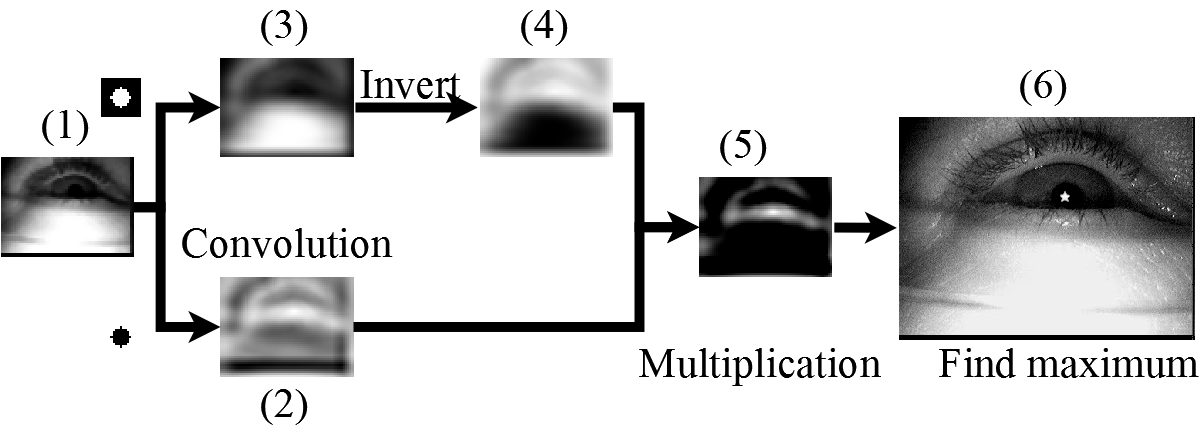
\includegraphics[width=0.8\linewidth]{img/ElSe}
	\caption{Ablauf der alternativen Berechnung zur Pupillen-Detektion von \cite{ElSe}}
	\label{img_else}
\end{figure}
\subsection{Ergebnisse}
Im Vergleich zu den anderen Verfahren im Test, ist ElSe in den meisten Fällen überlegen mit einer Verbesserung der Erkennungsrate um $14.53\%$ auf dem verwendeten Datensatz \cite{ElSe}.\\
Ein Problem entsteht wenn der Farbunterschied zwischen Iris und Pupille recht gering ausfällt oder durch Reflektionen der Kantenverlauf gestört wird.\\
Für die Anwendung ist der Bereich der Augen sehr klein und eine klare Detektion einzusprechend schwierig, wodurch vor allem die grobe Bestimmung der Ellipse von Interesse ist.